With its simple generic definition undirected graphical models have a lot of application areas. Starting from theoretically modeling physical interactions, like magnestism as mentioned in section \ref{sec:problem}, to more recent fields of research in the domains of information retrieval, natural language, speech (as for example in \cite{}) and image processing but also in the field of machine learning (as for example in \cite{}). In order to give a few examples of application this section introduces three examples, where Markov networks are utilized: section \ref{sec:term} describes how undirected graphical models are used to express term dependencies in the field of information retrieval, section \ref{sec:tag} shows an example of the application within the area of natural language processing by examining part-of-speechs, semantic role labels and more and last but not least section \ref{sec:image} describe a method of gaining a higher resoluted image by using Markov networks and training data.

\subsection{Information retrieval: Term Dependencies}
\label{sec:term}

TODO: forward and backward sources from this article \cite{metzler2005markov}
TODO: Get some more information from \href{http:\\www.slideplayer.com/slide/6012545}{Slides for this topic}

Donald Metzler and W. Bruce Croft describe in \cite{metzler2005markov} a model for term dependencies using a Markov network. Afterwards this model can be used for information retrieval.

As in this article indicated every term of the query is considered as a random variable and are linked to the document which shall be ranked. In addition to this Metzler and Croft distinguish into three different dependecy assumptions: full independecy, sequential independency and full dependency among the terms as illustrated in \ref{fig:termdep}. Sequential dependency means that only ancient terms of the query are dependent like in a bigram model, full independency means that all query terms are conditionally independent from one another and finally full dependency describes a model, in which all query terms are coniditionally dependened on each other. 

In order to apply this method for a query following steps must be taken:
\begin{enumerate}
\item represent the query term dependencies by a Markov network
\item define potential functions for the cliques of the network
\item compute the rank of each document $P_\Lambda (D|Q)$ and sort them in a descending order
\end{enumerate}

\begin{figure}[htpb]
  \centering
  	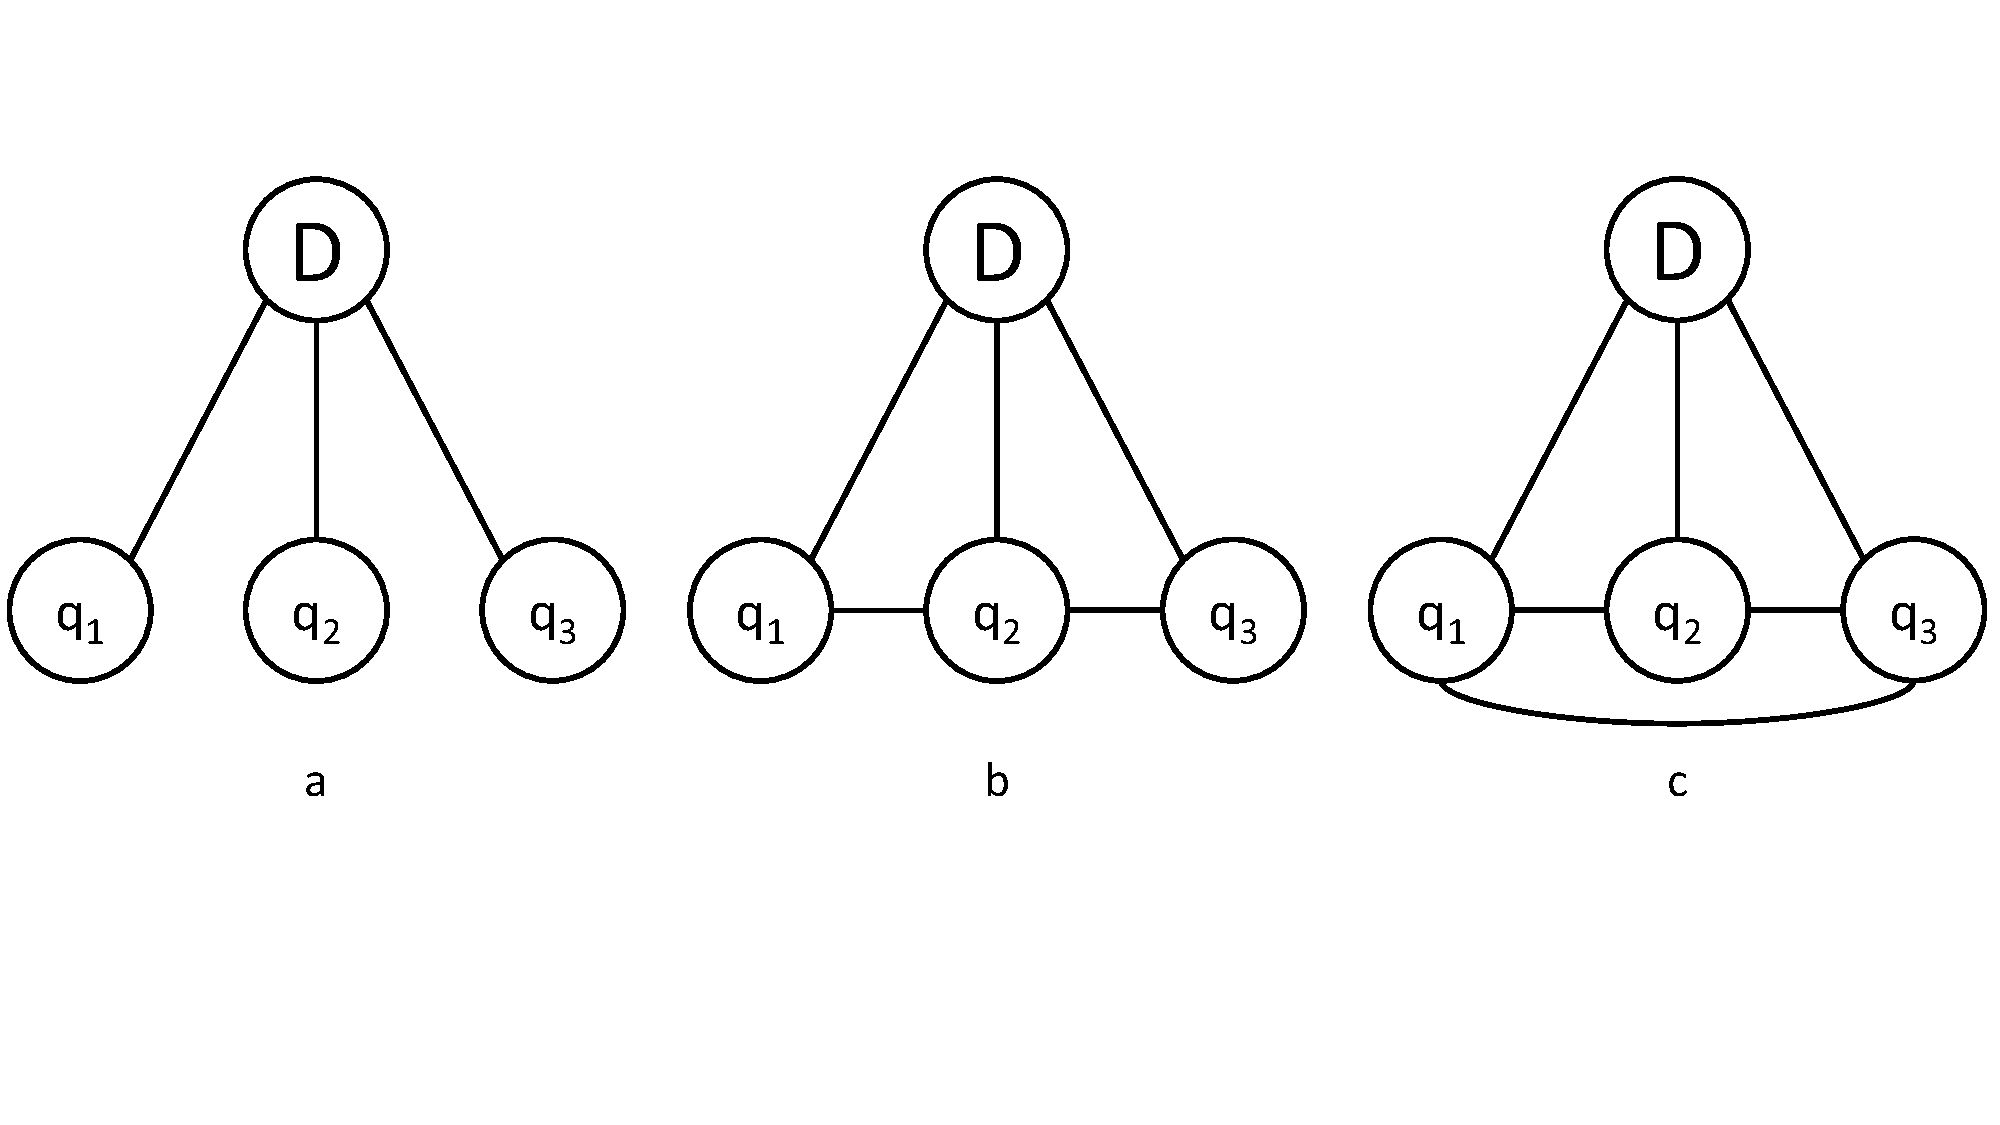
\includegraphics[scale=0.4]{img/termdep.pdf} 
  \caption{Dependency assumptions: a) full independency, b) sequential dependency and c) full dependency}
  \label{fig:termdep}
\end{figure}

Hereby D is a document, Q a query and $P_\Lambda$ a function which applies a weighted potential function to each clique of the Markov model. The potential functions can be considered as compatibility functions, as described in \ref{sec:methodology}, and are restriced to be strictly positive by \cite{metzler2005markov}. Further if full independency is assummed every term would form a smallest clique with the document under investigation and will lead to one contribution to the rank of the document with repect to the query. If elsewise full dependency is assummed, there are also cliques with all query terms and the document taken into account.

After experimenal testing on different data sets Metzler and Croft show the efficiency of this undirected graphical model approach in comparisson with other models like the bigram model. When comparing the three different independence assumptions the sequential dependecy assumption leads in terms of effectivity in contrast to the full independece assupmtion and also leads in terms of efficientcy and ad hoc requests in comparison with the full dependency assumption.


\subsection{Natural language processing: word tagging}
\label{sec:tag}

get some infos from \cite{collobert2011natural}


\subsection{Image processing: super-resolution}
\label{sec:image}

TODO: figure wich shows the method, described below

One application of markov networks in the field of image processing is the computation of a super-resolution of an image. This means that a low-resolution image can be converted into an high-resoultion image, for instance by using an already trained example database, as described in \cite{freeman2002example}. As Freeman describes, first an training dataset is build by mapping a high resolution patch (for example 16 pxiels x 16 pixels) of any image to a low resolution counter patch (for example 8 pixels x 8 pixels) in order to use the reversed mapping later to find a high-resolution patch for a low-resolution input patch. Thus after training, there should be in the best case multiple high-resolution patches for one low-resolution patch.

In the next step an low-resolution input image is fragmented into multiple patches, which are represented by nodes in the Markov network. Furthermore the target high-resolution patches are also nodes which are at this point linked to the input nodes. To examine which high-resolution patch fits best, they overlap with their neighbor by one pixel. Thus, the best value combination of target patches needs to be minimized in terms of the error of the overlapping pixels or maximized in the terms of probability, how "likely" the resulting image fits to the input image.
